
%(BEGIN_QUESTION)
% Copyright 2009, Tony R. Kuphaldt, released under the Creative Commons Attribution License (v 1.0)
% This means you may do almost anything with this work of mine, so long as you give me proper credit

This simplified PFD shows the {\it fluid catalytic cracking} or {\it FCC} process, used extensively in American oil refineries.  FCC processes employ finely-powdered catalyst to accelerate chemical reactions where heavy liquid hydrocarbon molecules are split (``cracked'') into lighter molecules, producing petroleum liquids with greater market value.  This is not unlike the chemical process of {\it biomass gasification}, where solid fuel materials are broken down by intense heat into simpler, flammable gases with more flexible application as fuels:

$$\includegraphics[width=15.5cm]{i00628x01.eps}$$

The cracking reactions begin in the riser and continue in the reactor, with the catalyst powder carried along by the steam and hydrocarbon fluids.  These reactions leave much of the catalyst powder covered with coke (solid carbon deposits) which limits its effectiveness as a catalyst.  This ``spent'' catalyst falls by gravity into the regenerator, where it encounters a blast of air entering the bottom of the vessel, converting the carbon deposits into CO and CO$_{2}$ gases and ``fluidizing'' the catalyst powder once again so it flows freely back to the riser.  The hot gases leaving the regenerator pass through a heat exchanger to boil water into useful steam, then pass to a burner where more air is introduced to convert the CO gas into CO$_{2}$ gas and generate more steam with the heat.  Vapors leaving the top of the reactor vessel are distilled into their constituent compounds in the fractionator vessel, with the heaviest of them recycled back to the reactor for re-processing.

\vskip 10pt

Identify whether the major chemical reactions are {\it exothermic} or {\it endothermic} in each of the following process vessels, explaining your rationale for each case:

\begin{itemize}
\item{} Reactor
\vskip 10pt
\item{} Regenerator
\vskip 10pt
\item{} CO boiler
\end{itemize}

\vfil

\underbar{file i00628}
\eject
%(END_QUESTION)





%(BEGIN_ANSWER)

This is a graded question -- no answers or hints given!

%(END_ANSWER)





%(BEGIN_NOTES)

\begin{itemize}
\item{} Reactor: {\it endothermic}, because the molecules are being split, and that requires an input of energy.  This energy is mostly supplied by the hot, regenerated catalyst coming down from the regenerator vessel as it contacts the fresh feed and recycle slurry entering the bottom of the riser.
\vskip 10pt
\item{} Regenerator: {\it exothermic}, because carbon (C) is being combusted with oxygen (O) to form carbon monoxide (CO) and carbon dioxide (CO$_{2}$) gases, both processes where atoms join to form molecules and release energy.
\vskip 10pt
\item{} CO boiler: {\it exothermic}, because carbon monoxide (CO) is being combusted with oxygen (O) to form carbon dioxide (CO$_{2}$) gas, a process where atoms join to form molecules and release energy.
\end{itemize}

In fact, the exothermic reactions inside the regenerator help drive the energy input requirement of the reactor, the hot ``regenerated'' catalyst carrying much of the combustion heat from inside the regenerator vessel to the riser and reactor vessels.

%INDEX% Chemistry, catalyst
%INDEX% Process: fluid catalytic cracker (oil refinery)

%(END_NOTES)


